\documentclass[11pt,]{article}
\usepackage{lmodern}
\usepackage{amssymb,amsmath}
\usepackage{ifxetex,ifluatex}
\usepackage{fixltx2e} % provides \textsubscript
\ifnum 0\ifxetex 1\fi\ifluatex 1\fi=0 % if pdftex
  \usepackage[T1]{fontenc}
  \usepackage[utf8]{inputenc}
\else % if luatex or xelatex
  \ifxetex
    \usepackage{mathspec}
    \usepackage{xltxtra,xunicode}
  \else
    \usepackage{fontspec}
  \fi
  \defaultfontfeatures{Mapping=tex-text,Scale=MatchLowercase}
  \newcommand{\euro}{€}
\fi
% use upquote if available, for straight quotes in verbatim environments
\IfFileExists{upquote.sty}{\usepackage{upquote}}{}
% use microtype if available
\IfFileExists{microtype.sty}{%
\usepackage{microtype}
\UseMicrotypeSet[protrusion]{basicmath} % disable protrusion for tt fonts
}{}
\usepackage[margin=1in]{geometry}
\usepackage{longtable,booktabs}
\usepackage{graphicx}
\makeatletter
\def\maxwidth{\ifdim\Gin@nat@width>\linewidth\linewidth\else\Gin@nat@width\fi}
\def\maxheight{\ifdim\Gin@nat@height>\textheight\textheight\else\Gin@nat@height\fi}
\makeatother
% Scale images if necessary, so that they will not overflow the page
% margins by default, and it is still possible to overwrite the defaults
% using explicit options in \includegraphics[width, height, ...]{}
\setkeys{Gin}{width=\maxwidth,height=\maxheight,keepaspectratio}
\ifxetex
  \usepackage[setpagesize=false, % page size defined by xetex
              unicode=false, % unicode breaks when used with xetex
              xetex]{hyperref}
\else
  \usepackage[unicode=true]{hyperref}
\fi
\hypersetup{breaklinks=true,
            bookmarks=true,
            pdfauthor={},
            pdftitle={},
            colorlinks=true,
            citecolor=blue,
            urlcolor=blue,
            linkcolor=magenta,
            pdfborder={0 0 0}}
\urlstyle{same}  % don't use monospace font for urls
\setlength{\parindent}{0pt}
\setlength{\parskip}{6pt plus 2pt minus 1pt}
\setlength{\emergencystretch}{3em}  % prevent overfull lines
\setcounter{secnumdepth}{0}

%%% Use protect on footnotes to avoid problems with footnotes in titles
\let\rmarkdownfootnote\footnote%
\def\footnote{\protect\rmarkdownfootnote}

%%% Change title format to be more compact
\usepackage{titling}

% Create subtitle command for use in maketitle
\newcommand{\subtitle}[1]{
  \posttitle{
    \begin{center}\large#1\end{center}
    }
}

\setlength{\droptitle}{-2em}
  \title{}
  \pretitle{\vspace{\droptitle}}
  \posttitle{}
  \author{}
  \preauthor{}\postauthor{}
  \date{}
  \predate{}\postdate{}

% load packages
\usepackage{amsmath,amsfonts,float,makecell,titletoc,tocloft,titlesec,natbib,pdfpages}
\usepackage[T1]{fontenc}
\usepackage{lmodern}
\usepackage[utf8]{inputenc}

% format captions
\usepackage[labelfont={small,bf}, labelsep=space, font={small}]{caption}

% format headings
\titleformat{\subsection}
{\normalfont\Large\bfseries}{\thesubsection}{1em}{}
\titleformat{\subsubsection}
{\normalfont\large\bfseries}{\thesubsubsection}{1em}{}
\titleformat{\paragraph}
{\normalfont\normalsize\bfseries}{\theparagraph}{1em}{}
\titleformat{\subparagraph}
{\normalfont\normalsize\itshape}{\thesubparagraph}{1em}{}

\titlespacing\paragraph{0pt}{12pt plus 4pt minus 2pt}{+0pt plus 2pt minus 2pt}
\titlespacing{\subparagraph}{0pt}{6pt plus 4pt minus 2pt}{+0pt plus 2pt minus 2pt}

% format toc
\renewcommand\cftsubsecfont{\normalfont\normalsize\bfseries}
% \renewcommand\cftsubsubsecfont{\normalfont\normalsize\bfseries}
% \renewcommand\cftparafont{\normalfont\normalsize\bfseries}
% \renewcommand\cftsubparafont{\normalfont\normalsize\itshape}

% make figures static
\let\origfigure\figure
\let\endorigfigure\endfigure
\renewenvironment{figure}[1][2] {
	\expandafter\origfigure\expandafter[H]
} {
	\endorigfigure
}


\begin{document}

\maketitle


\subsection{Supporting Information}\label{supporting-information}

\begin{figure}
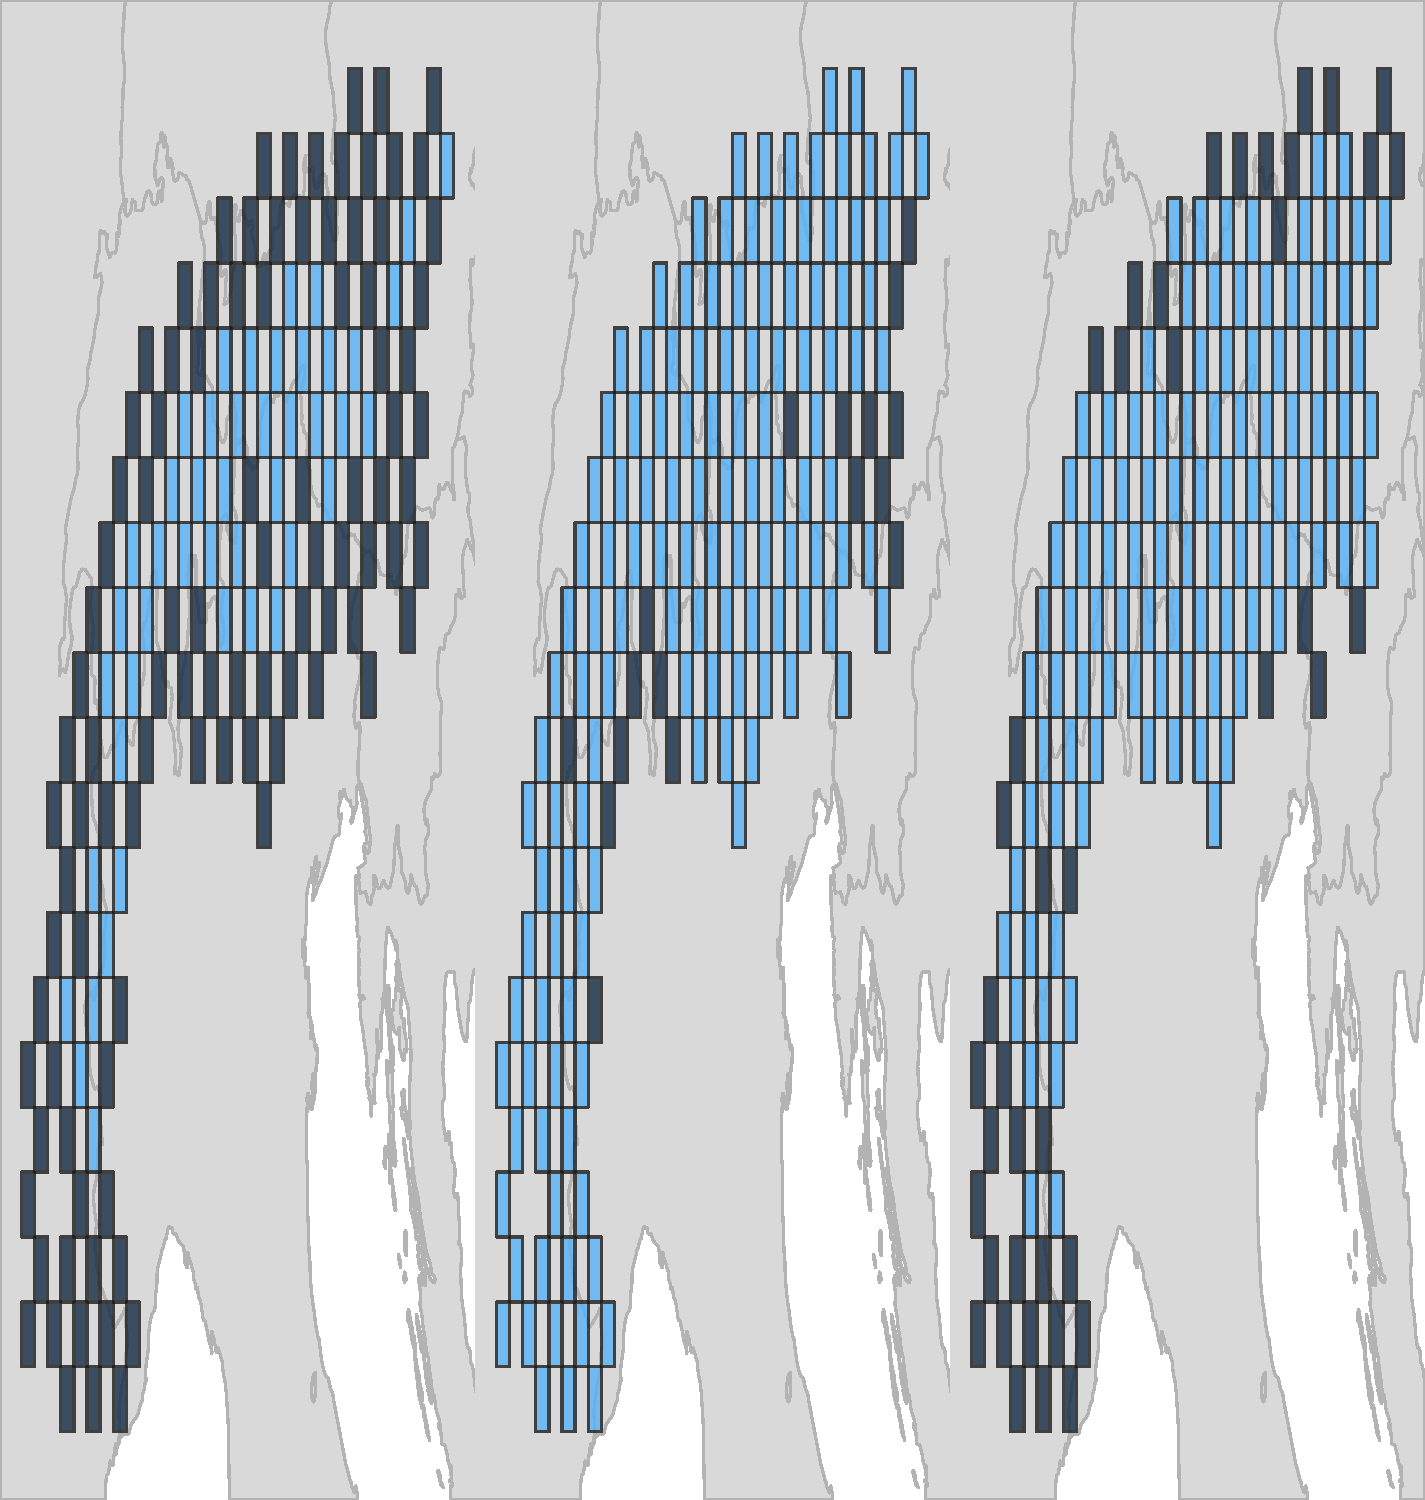
\includegraphics[width=7.5in,height=8.5in]{supporting_information_files/figure-latex/unnamed-chunk-2-1} \caption{Species distributions. Squares represent planning units. For a given species, planning units that were found to be inhabited are denoted with bright blue.}\label{fig:unnamed-chunk-2}
\end{figure}

\begin{figure}[htbp]
\centering
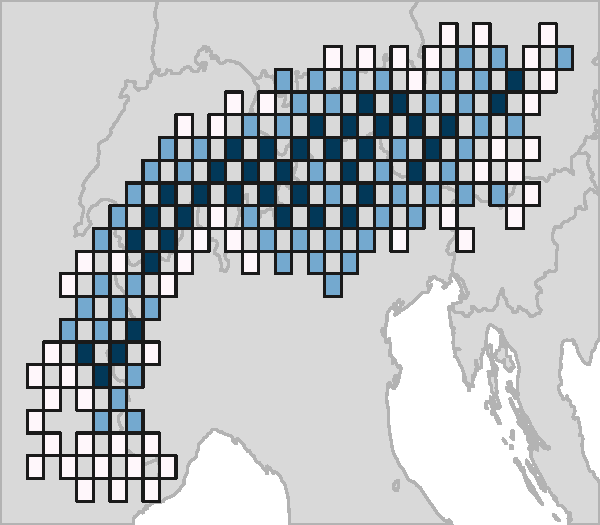
\includegraphics{supporting_information_files/figure-latex/unnamed-chunk-3-1.pdf}
\caption{Species richness. Squares denote planning units. Planning units
with a brighter color are inhabited by more species.}
\end{figure}

\begin{figure}[htbp]
\centering
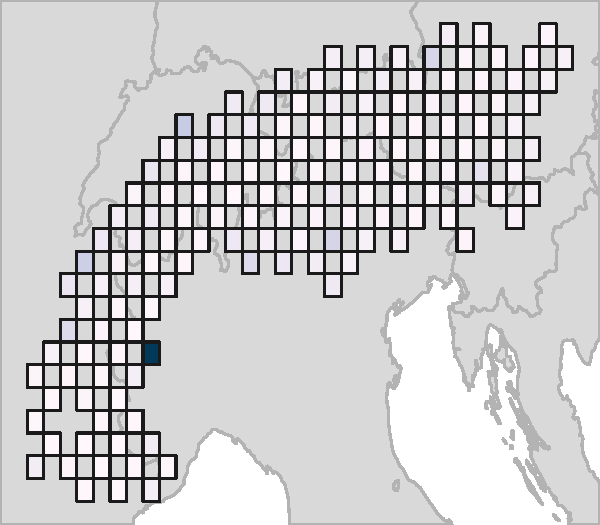
\includegraphics{supporting_information_files/figure-latex/unnamed-chunk-4-1.pdf}
\caption{Climatic variation. Each panel depicts variation based on a
different principle component (PC). Squares represent planning units.
The color of each planning unit denotes the average PC value of pixels
inside it. Planning units with more similar colors have more similar
climate regimes.}
\end{figure}

\begin{verbatim}
## Warning: Removed 6 rows containing missing values (geom_point).
\end{verbatim}

\begin{verbatim}
## Warning: Removed 2 rows containing missing values (geom_path).
\end{verbatim}

\begin{figure}[htbp]
\centering
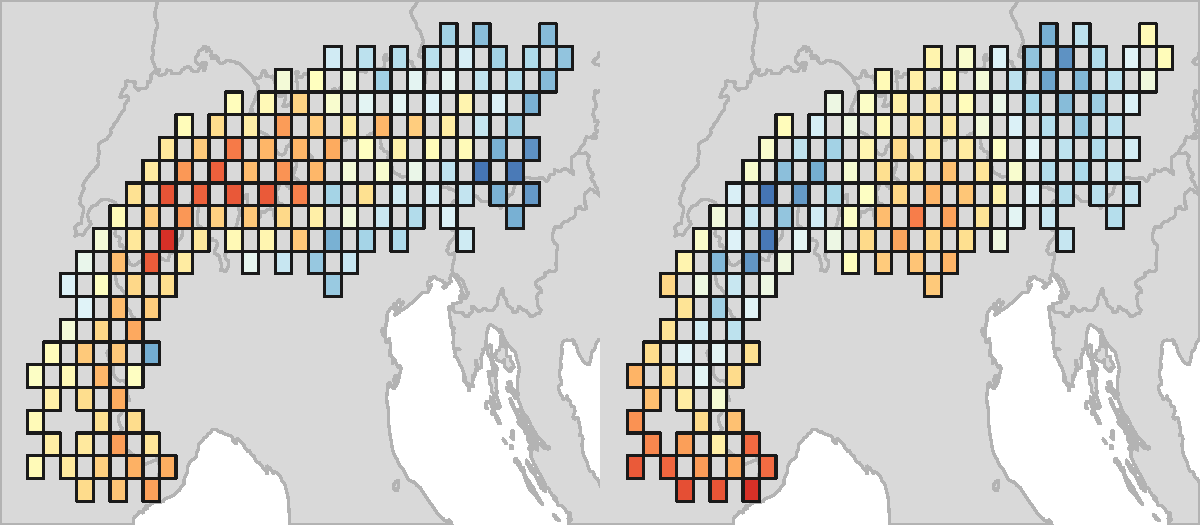
\includegraphics{supporting_information_files/figure-latex/unnamed-chunk-5-1.pdf}
\caption{Relative support ($\Delta$K) for the number of populations in
each species. Each panel denotes a different species. The number of
populations with the highest $Delta$K value is has the most support.}
\end{figure}

\begin{figure}[htbp]
\centering
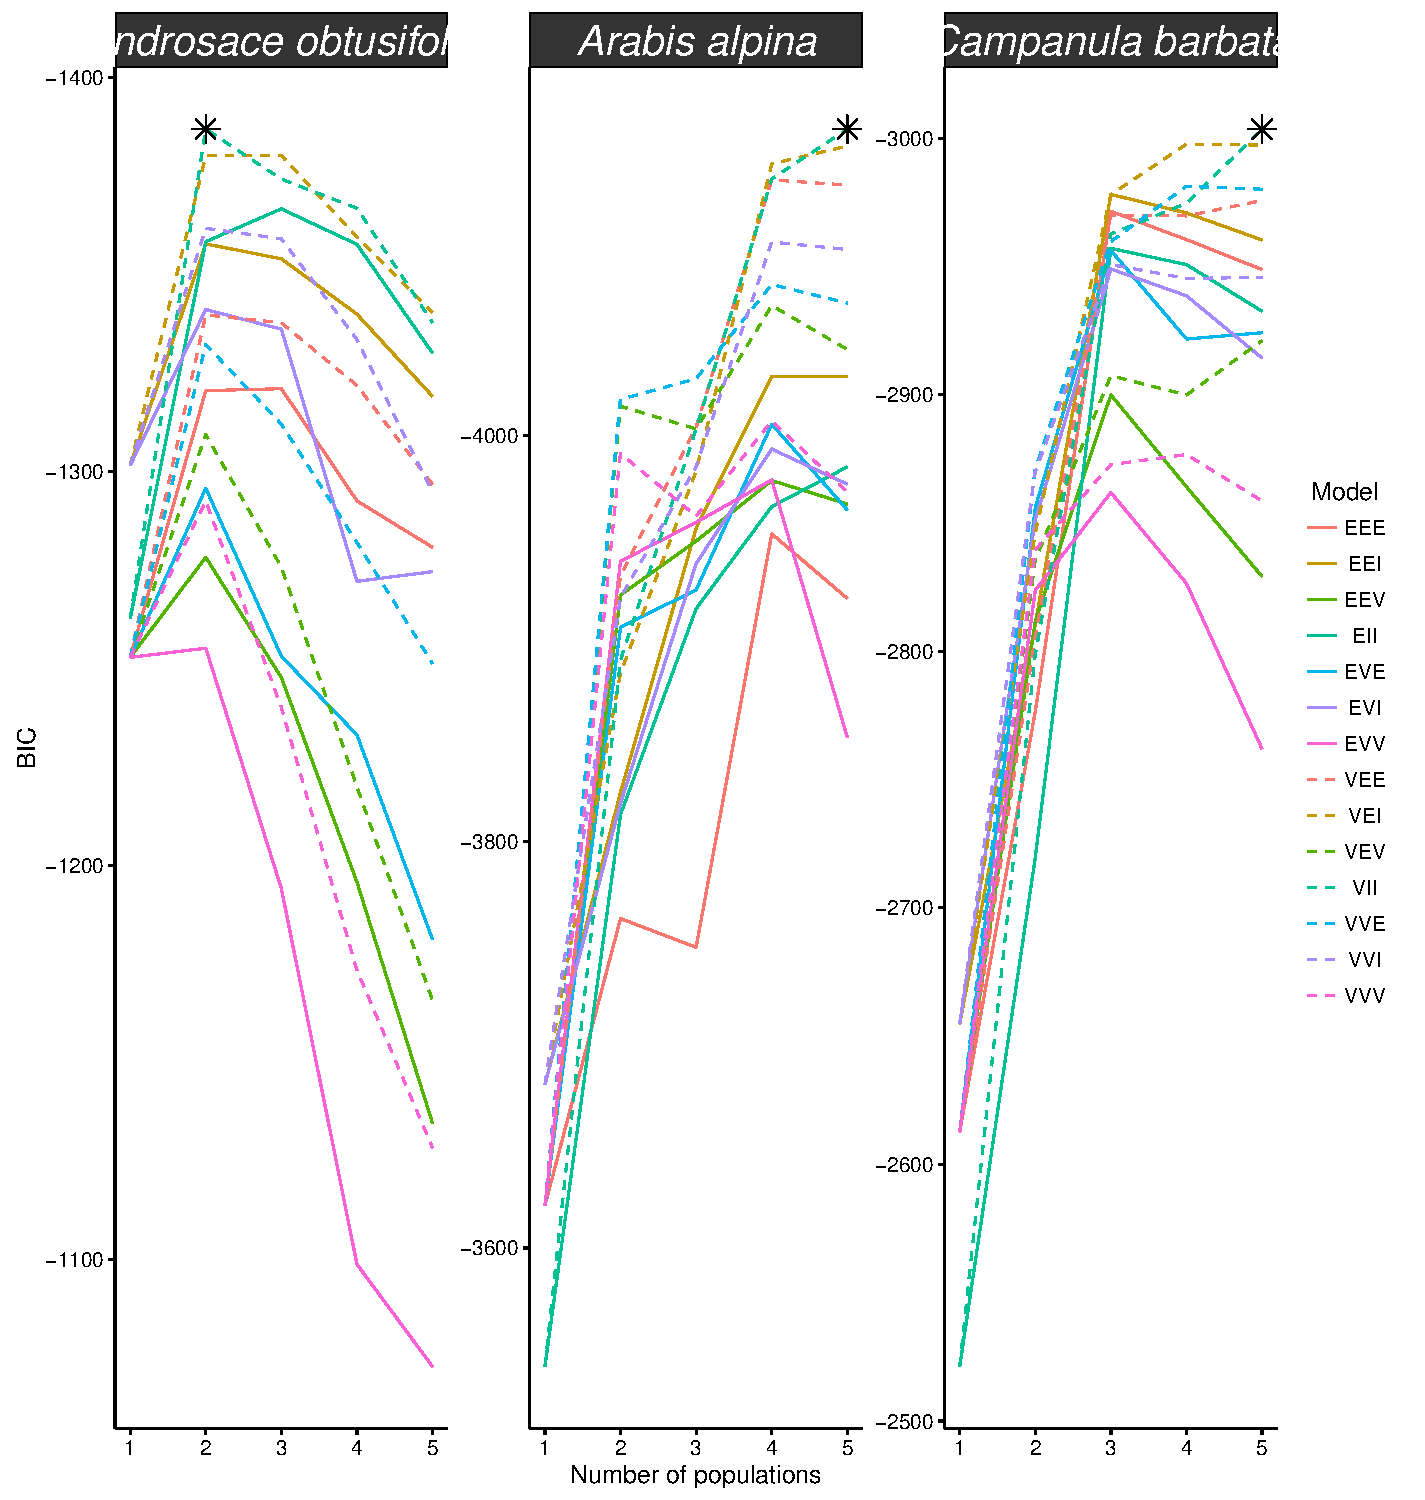
\includegraphics{supporting_information_files/figure-latex/unnamed-chunk-6-1.pdf}
\caption{Population membership plots. Each panel depicts a different
species. Each vertical bar represents a different individual. The colors
in each bar denote the probability that the individual belongs to
different populations.}
\end{figure}

\begin{figure}[htbp]
\centering
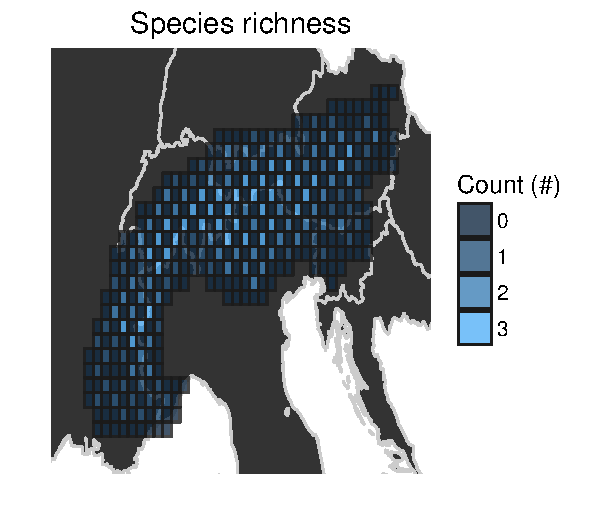
\includegraphics{supporting_information_files/figure-latex/unnamed-chunk-7-1.pdf}
\caption{Distribution of populations. Each panel depicts a different
species. Each pie chart represents a grid cell where individuals
belonging to a species were sampled. The colors of the pie chart show
the frequency of individuals belonging to different populations.}
\end{figure}

\begin{figure}[htbp]
\centering
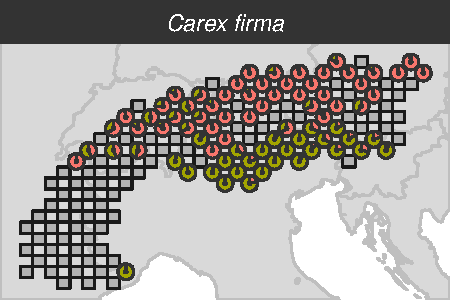
\includegraphics{supporting_information_files/figure-latex/unnamed-chunk-9-1.pdf}
\caption{Distribution of adaptive and neutral genetic variation in
\textit{Androsace obtusifolia}. Each square represents a planning unit.
The color of each planning unit panel corresponds to ordination values.
Planning units with similar colors contain individiduals with similar
genetic variation.}
\end{figure}

\begin{figure}[htbp]
\centering
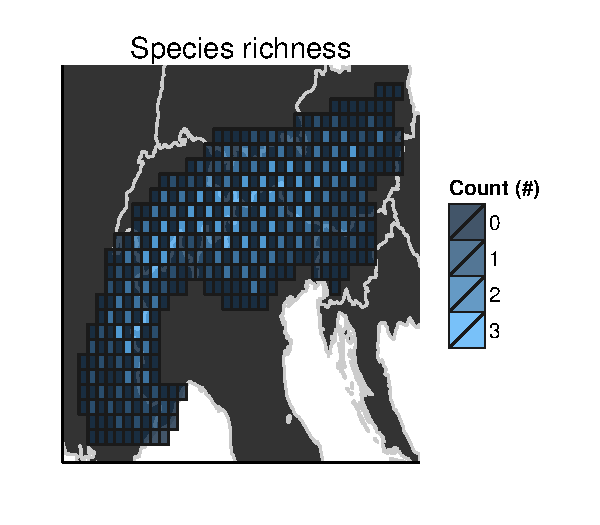
\includegraphics{supporting_information_files/figure-latex/unnamed-chunk-10-1.pdf}
\caption{Distribution of adaptive and neutral genetic variation in
\textit{Arabis alpina}. See Figure S6 caption for conventions.}
\end{figure}

\begin{figure}[htbp]
\centering
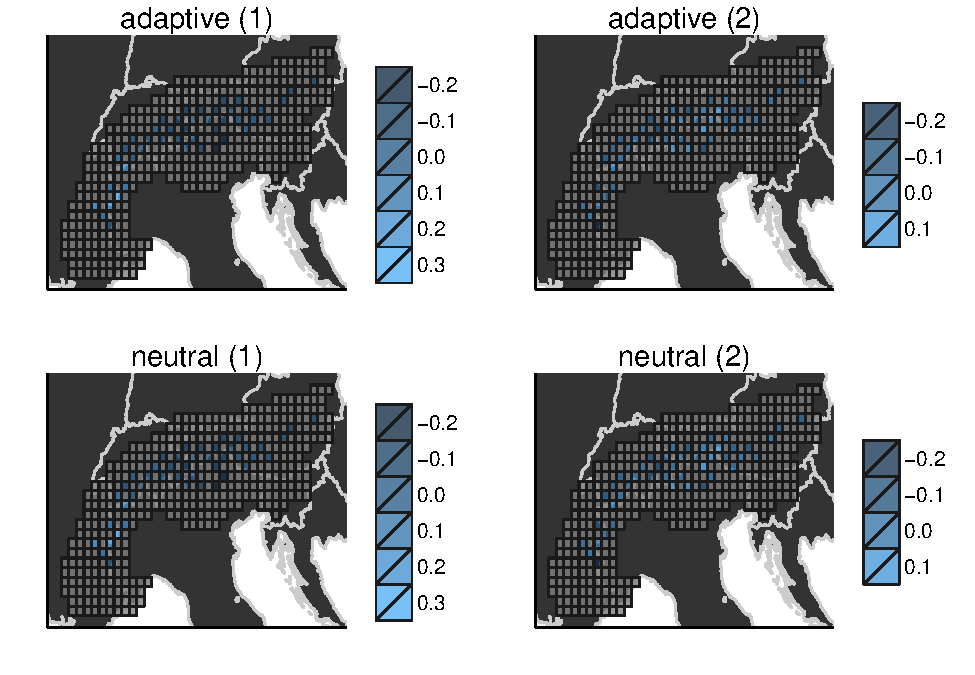
\includegraphics{supporting_information_files/figure-latex/unnamed-chunk-11-1.pdf}
\caption{Distribution of adaptive and neutral genetic variation in
\textit{Campanula barbata}. See Figure S6 caption for conventions.}
\end{figure}

\subsubsection{Table S1: Principle components analysis on climatic
variation}\label{table-s1-principle-components-analysis-on-climatic-variation}

\begin{longtable}[c]{@{}lccc@{}}
\toprule\addlinespace
Principle Component & Eigen Value & Variation explained (\%) &
Accumulative variation explained (\%)
\\\addlinespace
\midrule\endhead
1 & 216765.14 & 82.67 & 82.67
\\\addlinespace
2 & 38177.84 & 14.56 & 97.23
\\\addlinespace
3 & 5356.75 & 2.04 & 99.27
\\\addlinespace
4 & 1216.67 & 0.46 & 99.73
\\\addlinespace
5 & 700.39 & 0.27 & 100.00
\\\addlinespace
\bottomrule
\addlinespace
\caption{Summary of principle components analysis (PCA) on bioclimatic
variation across the study area. The first two principle components
(PCs) were used for subsequent analysis.}
\end{longtable}

\subsubsection{Table S2: BayeScan
Results}\label{table-s2-bayescan-results}

\begin{longtable}[c]{@{}lcccccc@{}}
\toprule\addlinespace
Species & Primer & Probability & q-value & $\alpha$ & $F_{ST}$ & Type
\\\addlinespace
\midrule\endhead
\textit{Androsace obtusifolia} & AAC\_CAN\_83.0 & 0.04 & 0.81 & -0.01 &
0.39 & neutral
\\\addlinespace
& AAC\_CAN\_85.0 & 0.04 & 0.81 & -0.01 & 0.39 & neutral
\\\addlinespace
& AAC\_CAN\_89.0 & 0.11 & 0.70 & -0.01 & 0.39 & neutral
\\\addlinespace
& AAC\_CAN\_91.0 & 0.04 & 0.80 & 0.00 & 0.39 & neutral
\\\addlinespace
& AAC\_CAN\_100.0 & 0.44 & 0.37 & -0.62 & 0.29 & neutral
\\\addlinespace
& AAC\_CAN\_102.0 & 0.07 & 0.76 & 0.00 & 0.39 & neutral
\\\addlinespace
& AAC\_CAN\_108.0 & 0.07 & 0.73 & -0.01 & 0.39 & neutral
\\\addlinespace
& AAC\_CAN\_124.0 & 0.15 & 0.63 & -0.07 & 0.37 & neutral
\\\addlinespace
& AAC\_CAN\_125.0 & 0.11 & 0.73 & -0.10 & 0.37 & adaptive
\\\addlinespace
& AAC\_CAN\_128.0 & 0.04 & 0.81 & 0.03 & 0.39 & neutral
\\\addlinespace
& AAC\_CAN\_130.0 & 0.48 & 0.34 & -0.10 & 0.38 & neutral
\\\addlinespace
& AAC\_CAN\_132.0 & 0.00 & 0.85 & 0.00 & 0.39 & neutral
\\\addlinespace
& AAC\_CAN\_133.0 & 0.11 & 0.71 & 0.00 & 0.39 & neutral
\\\addlinespace
& AAC\_CAN\_136.0 & 0.07 & 0.76 & -0.11 & 0.38 & neutral
\\\addlinespace
& AAC\_CAN\_137.0 & 0.15 & 0.65 & -0.07 & 0.38 & adaptive
\\\addlinespace
& AAC\_CAN\_146.0 & 0.04 & 0.80 & 0.03 & 0.39 & neutral
\\\addlinespace
& AAC\_CAN\_151.0 & 0.11 & 0.71 & 0.06 & 0.39 & neutral
\\\addlinespace
& AAC\_CAN\_152.0 & 0.00 & 0.85 & 0.00 & 0.39 & neutral
\\\addlinespace
& AAC\_CAN\_153.0 & 0.07 & 0.76 & 0.00 & 0.39 & neutral
\\\addlinespace
& AAC\_CAN\_182.0 & 0.04 & 0.81 & -0.10 & 0.37 & neutral
\\\addlinespace
& AAC\_CAN\_195.0 & 0.15 & 0.65 & -0.19 & 0.37 & adaptive
\\\addlinespace
& AAC\_CAN\_211.0 & 0.33 & 0.56 & -0.28 & 0.37 & neutral
\\\addlinespace
& AAC\_CAN\_220.0 & 0.15 & 0.65 & 0.00 & 0.39 & adaptive
\\\addlinespace
& AAC\_CAN\_231.0 & 0.07 & 0.76 & 0.06 & 0.40 & neutral
\\\addlinespace
& AAC\_CAN\_239.0 & 0.04 & 0.80 & -0.06 & 0.38 & neutral
\\\addlinespace
& AAC\_CAN\_272.0 & 0.11 & 0.66 & 0.14 & 0.41 & neutral
\\\addlinespace
& AAC\_CAN\_319.0 & 0.07 & 0.78 & -0.02 & 0.38 & neutral
\\\addlinespace
& ACA\_CAT\_81.0 & 0.04 & 0.81 & 0.03 & 0.39 & neutral
\\\addlinespace
& ACA\_CAT\_85.0 & 0.11 & 0.73 & -0.06 & 0.38 & adaptive
\\\addlinespace
& ACA\_CAT\_90.0 & 0.11 & 0.71 & -0.11 & 0.37 & neutral
\\\addlinespace
& ACA\_CAT\_97.0 & 0.11 & 0.68 & 0.07 & 0.40 & neutral
\\\addlinespace
& ACA\_CAT\_99.0 & 0.07 & 0.78 & 0.04 & 0.39 & neutral
\\\addlinespace
& ACA\_CAT\_100.0 & 0.07 & 0.78 & -0.06 & 0.38 & neutral
\\\addlinespace
& ACA\_CAT\_102.0 & 0.07 & 0.76 & 0.00 & 0.39 & neutral
\\\addlinespace
& ACA\_CAT\_103.0 & 0.37 & 0.54 & -0.11 & 0.37 & neutral
\\\addlinespace
& ACA\_CAT\_108.0 & 0.07 & 0.76 & -0.02 & 0.38 & neutral
\\\addlinespace
& ACA\_CAT\_120.0 & 0.11 & 0.68 & 0.00 & 0.39 & neutral
\\\addlinespace
& ACA\_CAT\_124.0 & 0.00 & 0.85 & 0.00 & 0.39 & neutral
\\\addlinespace
& ACA\_CAT\_126.0 & 0.30 & 0.47 & 0.47 & 0.47 & neutral
\\\addlinespace
& ACA\_CAT\_129.0 & 0.63 & 0.12 & -0.07 & 0.39 & adaptive
\\\addlinespace
& ACA\_CAT\_131.0 & 0.04 & 0.81 & 0.01 & 0.39 & neutral
\\\addlinespace
& ACA\_CAT\_133.0 & 0.07 & 0.76 & -0.05 & 0.38 & neutral
\\\addlinespace
& ACA\_CAT\_135.0 & 0.04 & 0.81 & 0.00 & 0.39 & neutral
\\\addlinespace
& ACA\_CAT\_140.0 & 0.07 & 0.75 & 0.01 & 0.39 & neutral
\\\addlinespace
& ACA\_CAT\_148.0 & 0.04 & 0.81 & 0.01 & 0.39 & neutral
\\\addlinespace
& ACA\_CAT\_152.0 & 0.07 & 0.72 & 0.01 & 0.39 & neutral
\\\addlinespace
& ACA\_CAT\_153.0 & 0.04 & 0.81 & -0.01 & 0.39 & neutral
\\\addlinespace
& ACA\_CAT\_155.0 & 0.41 & 0.48 & -0.83 & 0.27 & adaptive
\\\addlinespace
& ACA\_CAT\_157.0 & 0.00 & 0.85 & 0.00 & 0.39 & neutral
\\\addlinespace
& ACA\_CAT\_159.0 & 0.33 & 0.53 & -0.65 & 0.36 & neutral
\\\addlinespace
& ACA\_CAT\_162.0 & 0.33 & 0.57 & 0.30 & 0.43 & neutral
\\\addlinespace
& ACA\_CAT\_168.0 & 0.00 & 0.85 & 0.00 & 0.39 & neutral
\\\addlinespace
& ACA\_CAT\_173.0 & 0.11 & 0.68 & -0.08 & 0.38 & neutral
\\\addlinespace
& ACA\_CAT\_177.0 & 0.04 & 0.80 & 0.00 & 0.39 & neutral
\\\addlinespace
& ACA\_CAT\_178.0 & 0.07 & 0.76 & -0.02 & 0.38 & neutral
\\\addlinespace
& ACA\_CAT\_187.0 & 0.07 & 0.72 & 0.00 & 0.39 & neutral
\\\addlinespace
& ACA\_CAT\_192.0 & 0.07 & 0.72 & 0.06 & 0.39 & neutral
\\\addlinespace
& ACA\_CAT\_196.0 & 0.37 & 0.53 & -0.45 & 0.32 & neutral
\\\addlinespace
& ACA\_CAT\_199.0 & 0.07 & 0.73 & 0.03 & 0.39 & neutral
\\\addlinespace
& ACA\_CAT\_200.0 & 0.11 & 0.73 & -0.03 & 0.38 & adaptive
\\\addlinespace
& ACA\_CAT\_204.0 & 0.00 & 0.85 & 0.00 & 0.39 & neutral
\\\addlinespace
& ACA\_CAT\_205.0 & 0.37 & 0.53 & -0.54 & 0.30 & neutral
\\\addlinespace
& ACA\_CAT\_210.0 & 0.44 & 0.41 & -0.30 & 0.34 & adaptive
\\\addlinespace
& ACA\_CAT\_214.0 & 0.11 & 0.73 & -0.04 & 0.38 & adaptive
\\\addlinespace
& ACA\_CAT\_219.0 & 0.11 & 0.70 & 0.00 & 0.39 & neutral
\\\addlinespace
& ACA\_CAT\_229.0 & 0.44 & 0.40 & -0.48 & 0.32 & adaptive
\\\addlinespace
& ACA\_CAT\_237.0 & 0.00 & 0.85 & 0.00 & 0.39 & neutral
\\\addlinespace
& ACA\_CAT\_243.0 & 0.22 & 0.50 & -0.04 & 0.38 & adaptive
\\\addlinespace
& ACA\_CAT\_246.0 & 0.15 & 0.64 & -0.03 & 0.38 & neutral
\\\addlinespace
& ACA\_CAT\_248.0 & 0.37 & 0.53 & 0.25 & 0.42 & neutral
\\\addlinespace
& ACA\_CAT\_282.0 & 0.00 & 0.85 & 0.00 & 0.39 & neutral
\\\addlinespace
& ACA\_CAT\_300.0 & 0.04 & 0.81 & -0.01 & 0.39 & neutral
\\\addlinespace
& ACA\_CAT\_390.0 & 0.11 & 0.71 & -0.09 & 0.37 & neutral
\\\addlinespace
& ACA\_CAT\_391.0 & 0.04 & 0.81 & -0.02 & 0.38 & neutral
\\\addlinespace
& ACA\_CAT\_393.0 & 0.22 & 0.55 & 0.14 & 0.41 & adaptive
\\\addlinespace
& AGG\_CAA\_82.3 & 0.11 & 0.70 & -0.05 & 0.38 & neutral
\\\addlinespace
& AGG\_CAA\_83.0 & 0.15 & 0.65 & -0.08 & 0.38 & adaptive
\\\addlinespace
& AGG\_CAA\_84.2 & 0.15 & 0.62 & 0.09 & 0.40 & neutral
\\\addlinespace
& AGG\_CAA\_86.9 & 0.04 & 0.81 & -0.02 & 0.38 & neutral
\\\addlinespace
& AGG\_CAA\_90.9 & 0.22 & 0.51 & -0.07 & 0.38 & neutral
\\\addlinespace
& AGG\_CAA\_94.8 & 0.41 & 0.49 & -0.50 & 0.32 & adaptive
\\\addlinespace
& AGG\_CAA\_95.6 & 0.07 & 0.76 & -0.04 & 0.38 & neutral
\\\addlinespace
& AGG\_CAA\_100.0 & 0.15 & 0.66 & -0.01 & 0.39 & adaptive
\\\addlinespace
& AGG\_CAA\_101.0 & 0.15 & 0.63 & 0.12 & 0.41 & neutral
\\\addlinespace
& AGG\_CAA\_109.3 & 0.07 & 0.73 & -0.01 & 0.38 & neutral
\\\addlinespace
& AGG\_CAA\_110.2 & 0.37 & 0.53 & -0.43 & 0.32 & neutral
\\\addlinespace
& AGG\_CAA\_113.5 & 0.00 & 0.85 & 0.00 & 0.39 & neutral
\\\addlinespace
& AGG\_CAA\_115.9 & 0.26 & 0.58 & -0.15 & 0.37 & neutral
\\\addlinespace
& AGG\_CAA\_117.4 & 0.15 & 0.64 & -0.18 & 0.36 & neutral
\\\addlinespace
& AGG\_CAA\_118.2 & 0.19 & 0.57 & -0.24 & 0.36 & adaptive
\\\addlinespace
& AGG\_CAA\_122.9 & 0.15 & 0.63 & NaN & NaN & neutral
\\\addlinespace
& AGG\_CAA\_129.5 & 0.48 & 0.34 & -0.18 & 0.36 & adaptive
\\\addlinespace
& AGG\_CAA\_130.1 & 0.15 & 0.64 & -0.02 & 0.38 & neutral
\\\addlinespace
& AGG\_CAA\_135.5 & 0.33 & 0.57 & -0.32 & 0.34 & neutral
\\\addlinespace
& AGG\_CAA\_137.9 & 0.15 & 0.61 & -0.11 & 0.37 & neutral
\\\addlinespace
& AGG\_CAA\_144.9 & 0.11 & 0.71 & 0.03 & 0.39 & neutral
\\\addlinespace
& AGG\_CAA\_145.8 & 0.15 & 0.64 & -0.06 & 0.38 & neutral
\\\addlinespace
& AGG\_CAA\_150.9 & 0.33 & 0.56 & -0.04 & 0.38 & neutral
\\\addlinespace
& AGG\_CAA\_152.8 & 0.19 & 0.56 & -0.06 & 0.38 & neutral
\\\addlinespace
& AGG\_CAA\_155.4 & 0.41 & 0.47 & -0.34 & 0.34 & neutral
\\\addlinespace
& AGG\_CAA\_164.0 & 0.33 & 0.57 & 0.35 & 0.44 & neutral
\\\addlinespace
& AGG\_CAA\_175.9 & 0.04 & 0.81 & 0.00 & 0.39 & neutral
\\\addlinespace
& AGG\_CAA\_181.6 & 0.22 & 0.51 & -0.06 & 0.38 & adaptive
\\\addlinespace
& AGG\_CAA\_182.1 & 0.00 & 0.85 & 0.00 & 0.39 & neutral
\\\addlinespace
& AGG\_CAA\_188.1 & 0.11 & 0.71 & 0.00 & 0.39 & neutral
\\\addlinespace
& AGG\_CAA\_191.3 & 0.70 & 0.24 & -0.46 & 0.34 & adaptive
\\\addlinespace
& AGG\_CAA\_193.9 & 0.00 & 0.85 & 0.00 & 0.39 & neutral
\\\addlinespace
& AGG\_CAA\_196.8 & 0.15 & 0.62 & 0.05 & 0.40 & neutral
\\\addlinespace
& AGG\_CAA\_201.7 & 0.11 & 0.73 & -0.05 & 0.38 & adaptive
\\\addlinespace
& AGG\_CAA\_212.4 & 0.41 & 0.47 & -0.06 & 0.38 & neutral
\\\addlinespace
& AGG\_CAA\_215.6 & 0.00 & 0.85 & 0.00 & 0.39 & neutral
\\\addlinespace
& AGG\_CAA\_219.0 & 0.04 & 0.81 & 0.00 & 0.39 & neutral
\\\addlinespace
& AGG\_CAA\_225.2 & 0.07 & 0.76 & 0.03 & 0.39 & neutral
\\\addlinespace
& AGG\_CAA\_253.2 & 0.00 & 0.85 & 0.00 & 0.39 & neutral
\\\addlinespace
& AGG\_CAA\_256.7 & 0.07 & 0.75 & -0.02 & 0.38 & neutral
\\\addlinespace
& AGG\_CAA\_262.5 & 0.11 & 0.73 & -0.02 & 0.38 & adaptive
\\\addlinespace
& AGG\_CAA\_263.6 & 0.44 & 0.42 & -0.16 & 0.37 & adaptive
\\\addlinespace
& AGG\_CAA\_264.8 & 0.11 & 0.70 & -0.15 & 0.37 & neutral
\\\addlinespace
& AGG\_CAA\_267.9 & 0.04 & 0.80 & -0.01 & 0.39 & neutral
\\\addlinespace
& AGG\_CAA\_269.8 & 0.41 & 0.49 & -0.22 & 0.38 & adaptive
\\\addlinespace
& AGG\_CAA\_270.8 & 0.07 & 0.75 & -0.05 & 0.38 & neutral
\\\addlinespace
& AGG\_CAA\_276.8 & 0.07 & 0.72 & 0.01 & 0.39 & neutral
\\\addlinespace
& AGG\_CAA\_299.0 & 0.33 & 0.50 & -0.29 & 0.37 & adaptive
\\\addlinespace
& AGG\_CAA\_305.1 & 0.04 & 0.81 & 0.00 & 0.39 & neutral
\\\addlinespace
& AGG\_CAA\_312.1 & 0.04 & 0.81 & -0.03 & 0.38 & neutral
\\\addlinespace
& AGG\_CAA\_313.2 & 0.11 & 0.70 & -0.18 & 0.36 & neutral
\\\addlinespace
& AGG\_CAA\_316.0 & 0.11 & 0.68 & -0.12 & 0.37 & neutral
\\\addlinespace
& AGG\_CAA\_319.0 & 0.07 & 0.76 & -0.04 & 0.38 & neutral
\\\addlinespace
& AGG\_CAA\_324.1 & 0.07 & 0.76 & 0.00 & 0.39 & neutral
\\\addlinespace
& AGG\_CAA\_359.4 & 0.37 & 0.52 & 0.32 & 0.44 & neutral
\\\addlinespace
& AGG\_CAA\_360.5 & 0.07 & 0.78 & 0.02 & 0.39 & neutral
\\\addlinespace
& AGG\_CAA\_363.2 & 0.07 & 0.73 & -0.04 & 0.38 & neutral
\\\addlinespace
& AGG\_CAA\_364.1 & 0.15 & 0.63 & NaN & NaN & neutral
\\\addlinespace
& AGG\_CAA\_376.2 & 0.11 & 0.71 & -0.08 & 0.38 & neutral
\\\addlinespace
& AGG\_CAA\_376.7 & 0.07 & 0.76 & -0.10 & 0.38 & neutral
\\\addlinespace
& AGG\_CAA\_396.0 & 0.15 & 0.64 & -0.09 & 0.37 & neutral
\\\addlinespace
& AGG\_CAA\_403.4 & 0.04 & 0.81 & 0.03 & 0.39 & neutral
\\\addlinespace
& AGG\_CAA\_420.5 & 0.48 & 0.32 & -0.03 & 0.38 & neutral
\\\addlinespace
\textit{Arabis alpina} & AAT\_CAC\_51.9 & 0.04 & 0.80 & 0.00 & 0.19 &
neutral
\\\addlinespace
& AAT\_CAC\_54.7 & 0.00 & 0.84 & 0.00 & 0.19 & neutral
\\\addlinespace
& AAT\_CAC\_69.0 & 0.44 & 0.38 & -0.12 & 0.17 & adaptive
\\\addlinespace
& AAT\_CAC\_73.6 & 0.11 & 0.67 & 0.06 & 0.20 & neutral
\\\addlinespace
& AAT\_CAC\_77.9 & 0.15 & 0.62 & 0.00 & 0.19 & adaptive
\\\addlinespace
& AAT\_CAC\_86.9 & 0.33 & 0.57 & -0.78 & 0.17 & neutral
\\\addlinespace
& AAT\_CAC\_90.5 & 0.04 & 0.80 & 0.01 & 0.19 & neutral
\\\addlinespace
& AAT\_CAC\_95.3 & 0.15 & 0.62 & 0.10 & 0.20 & adaptive
\\\addlinespace
& AAT\_CAC\_97.0 & 0.07 & 0.70 & 0.02 & 0.19 & neutral
\\\addlinespace
& AAT\_CAC\_97.1 & 0.37 & 0.51 & -0.20 & 0.16 & neutral
\\\addlinespace
& AAT\_CAC\_100.3 & 0.07 & 0.75 & 0.03 & 0.20 & neutral
\\\addlinespace
& AAT\_CAC\_105.4 & 0.00 & 0.84 & 0.00 & 0.19 & neutral
\\\addlinespace
& AAT\_CAC\_118.4 & 0.37 & 0.52 & 0.55 & 0.24 & neutral
\\\addlinespace
& AAT\_CAC\_121.3 & 0.04 & 0.79 & -0.02 & 0.19 & neutral
\\\addlinespace
& AAT\_CAC\_128.0 & 0.11 & 0.66 & 0.16 & 0.22 & neutral
\\\addlinespace
& AAT\_CAC\_130.0 & 0.07 & 0.73 & -0.02 & 0.19 & neutral
\\\addlinespace
& AAT\_CAC\_147.4 & 0.00 & 0.84 & 0.00 & 0.19 & neutral
\\\addlinespace
& AAT\_CAC\_156.9 & 0.41 & 0.44 & -0.24 & 0.15 & neutral
\\\addlinespace
& AAT\_CAC\_175.1 & 0.41 & 0.46 & -0.33 & 0.18 & adaptive
\\\addlinespace
& AAT\_CAC\_177.9 & 0.22 & 0.51 & 0.15 & 0.22 & neutral
\\\addlinespace
& AAT\_CAC\_179.6 & 0.15 & 0.61 & -0.02 & 0.19 & neutral
\\\addlinespace
& AAT\_CAC\_188.6 & 0.07 & 0.73 & -0.02 & 0.19 & neutral
\\\addlinespace
& AAT\_CAC\_190.0 & 0.07 & 0.73 & 0.04 & 0.20 & neutral
\\\addlinespace
& AAT\_CAC\_195.5 & 0.07 & 0.74 & -0.10 & 0.18 & neutral
\\\addlinespace
& AAT\_CAC\_197.1 & 0.04 & 0.80 & 0.01 & 0.19 & neutral
\\\addlinespace
& AAT\_CAC\_200.6 & 0.41 & 0.42 & -0.16 & 0.16 & neutral
\\\addlinespace
& AAT\_CAC\_201.8 & 0.07 & 0.73 & 0.02 & 0.19 & neutral
\\\addlinespace
& AAT\_CAC\_209.2 & 0.07 & 0.74 & 0.04 & 0.20 & neutral
\\\addlinespace
& AAT\_CAC\_213.1 & 0.33 & 0.55 & -0.20 & 0.18 & neutral
\\\addlinespace
& AAT\_CAC\_215.0 & 0.33 & 0.56 & -0.03 & 0.19 & neutral
\\\addlinespace
& AAT\_CAC\_216.2 & 0.00 & 0.84 & 0.00 & 0.19 & neutral
\\\addlinespace
& AAT\_CAC\_217.0 & 0.11 & 0.64 & -0.05 & 0.18 & neutral
\\\addlinespace
& AAT\_CAC\_218.1 & 0.07 & 0.73 & 0.01 & 0.19 & neutral
\\\addlinespace
& AAT\_CAC\_219.1 & 0.07 & 0.72 & 0.07 & 0.20 & neutral
\\\addlinespace
& AAT\_CAC\_225.5 & 0.04 & 0.78 & 0.01 & 0.19 & neutral
\\\addlinespace
& AAT\_CAC\_227.1 & 0.11 & 0.67 & 0.02 & 0.19 & neutral
\\\addlinespace
& AAT\_CAC\_229.1 & 0.11 & 0.69 & -0.02 & 0.19 & adaptive
\\\addlinespace
& AAT\_CAC\_231.4 & 0.15 & 0.59 & 0.11 & 0.21 & neutral
\\\addlinespace
& AAT\_CAC\_249.7 & 0.15 & 0.60 & 0.18 & 0.23 & neutral
\\\addlinespace
& AAT\_CAC\_259.3 & 0.19 & 0.56 & 0.15 & 0.22 & neutral
\\\addlinespace
& AAT\_CAC\_277.3 & 0.59 & 0.29 & 0.10 & 0.18 & neutral
\\\addlinespace
& AAT\_CAC\_298.1 & 0.37 & 0.51 & 0.43 & 0.24 & neutral
\\\addlinespace
& AAT\_CAC\_315.9 & 0.37 & 0.51 & -0.39 & 0.13 & neutral
\\\addlinespace
& AAT\_CAC\_330.4 & 0.33 & 0.57 & -0.17 & 0.19 & neutral
\\\addlinespace
& AAT\_CAC\_334.8 & 0.04 & 0.80 & -0.04 & 0.19 & neutral
\\\addlinespace
& AAT\_CAC\_336.6 & 0.07 & 0.69 & -0.14 & 0.17 & neutral
\\\addlinespace
& AAT\_CAC\_353.0 & 0.04 & 0.79 & 0.03 & 0.20 & neutral
\\\addlinespace
& AAT\_CAC\_359.2 & 0.00 & 0.84 & 0.00 & 0.19 & neutral
\\\addlinespace
& AAT\_CAC\_399.9 & 0.07 & 0.72 & 0.07 & 0.20 & neutral
\\\addlinespace
& AAT\_CAC\_410.5 & 0.19 & 0.59 & NaN & NaN & neutral
\\\addlinespace
& AAT\_CAC\_412.4 & 0.37 & 0.49 & -0.16 & 0.19 & neutral
\\\addlinespace
& AAT\_CAC\_458.1 & 0.00 & 0.84 & 0.00 & 0.19 & neutral
\\\addlinespace
& AAT\_CAC\_488.6 & 0.04 & 0.78 & 0.01 & 0.19 & neutral
\\\addlinespace
& AGT\_CAC\_53.8 & 0.04 & 0.79 & 0.02 & 0.19 & neutral
\\\addlinespace
& AGT\_CAC\_56.3 & 0.04 & 0.80 & 0.05 & 0.20 & neutral
\\\addlinespace
& AGT\_CAC\_98.2 & 0.19 & 0.56 & -0.08 & 0.18 & neutral
\\\addlinespace
& AGT\_CAC\_104.9 & 0.00 & 0.84 & 0.00 & 0.19 & neutral
\\\addlinespace
& AGT\_CAC\_114.8 & 0.11 & 0.67 & -0.09 & 0.18 & neutral
\\\addlinespace
& AGT\_CAC\_145.8 & 0.11 & 0.65 & 0.07 & 0.20 & neutral
\\\addlinespace
& AGT\_CAC\_154.2 & 0.44 & 0.38 & -0.13 & 0.19 & adaptive
\\\addlinespace
& AGT\_CAC\_158.1 & 0.04 & 0.80 & -0.01 & 0.19 & neutral
\\\addlinespace
& AGT\_CAC\_169.0 & 0.07 & 0.72 & 0.06 & 0.19 & neutral
\\\addlinespace
& AGT\_CAC\_171.1 & 0.44 & 0.36 & 0.31 & 0.26 & neutral
\\\addlinespace
& AGT\_CAC\_181.1 & 0.07 & 0.74 & 0.00 & 0.19 & neutral
\\\addlinespace
& AGT\_CAC\_183.0 & 0.07 & 0.72 & 0.05 & 0.19 & neutral
\\\addlinespace
& AGT\_CAC\_184.4 & 0.48 & 0.32 & 0.13 & 0.20 & adaptive
\\\addlinespace
& AGT\_CAC\_191.2 & 0.30 & 0.39 & -0.16 & 0.20 & adaptive
\\\addlinespace
& AGT\_CAC\_195.0 & 0.04 & 0.80 & 0.00 & 0.19 & neutral
\\\addlinespace
& AGT\_CAC\_200.9 & 0.00 & 0.84 & 0.00 & 0.19 & neutral
\\\addlinespace
& AGT\_CAC\_203.8 & 0.33 & 0.57 & 0.27 & 0.21 & neutral
\\\addlinespace
& AGT\_CAC\_205.8 & 0.15 & 0.62 & -0.04 & 0.19 & adaptive
\\\addlinespace
& AGT\_CAC\_210.0 & 0.07 & 0.70 & -0.06 & 0.19 & neutral
\\\addlinespace
& AGT\_CAC\_230.8 & 0.04 & 0.78 & 0.02 & 0.20 & neutral
\\\addlinespace
& AGT\_CAC\_241.0 & 0.19 & 0.52 & -0.05 & 0.18 & neutral
\\\addlinespace
& AGT\_CAC\_245.6 & 0.04 & 0.80 & 0.01 & 0.19 & neutral
\\\addlinespace
& AGT\_CAC\_264.7 & 0.37 & 0.49 & 0.09 & 0.21 & neutral
\\\addlinespace
& AGT\_CAC\_266.9 & 0.19 & 0.53 & 0.04 & 0.19 & neutral
\\\addlinespace
& AGT\_CAC\_269.4 & 0.22 & 0.53 & 0.19 & 0.21 & adaptive
\\\addlinespace
& AGT\_CAC\_274.0 & 0.04 & 0.79 & -0.01 & 0.19 & neutral
\\\addlinespace
& AGT\_CAC\_285.6 & 0.07 & 0.74 & 0.00 & 0.19 & neutral
\\\addlinespace
& AGT\_CAC\_291.5 & 0.00 & 0.84 & 0.00 & 0.19 & neutral
\\\addlinespace
& AGT\_CAC\_295.6 & 0.15 & 0.64 & 0.10 & 0.20 & neutral
\\\addlinespace
& AGT\_CAC\_315.2 & 0.07 & 0.74 & 0.00 & 0.19 & neutral
\\\addlinespace
& AGT\_CAC\_332.1 & 0.37 & 0.51 & 0.09 & 0.21 & neutral
\\\addlinespace
& AGT\_CAC\_347.8 & 0.04 & 0.80 & 0.03 & 0.19 & neutral
\\\addlinespace
& AGT\_CAC\_355.2 & 0.19 & 0.56 & -0.08 & 0.18 & neutral
\\\addlinespace
& AGT\_CAC\_360.2 & 0.07 & 0.75 & 0.03 & 0.20 & neutral
\\\addlinespace
& AGT\_CAC\_386.5 & 0.41 & 0.45 & -0.55 & 0.15 & adaptive
\\\addlinespace
& AGT\_CAC\_418.5 & 0.00 & 0.84 & 0.00 & 0.19 & neutral
\\\addlinespace
& AGT\_CAC\_420.2 & 0.07 & 0.73 & 0.04 & 0.20 & neutral
\\\addlinespace
& AGT\_CAC\_444.3 & 0.26 & 0.53 & 0.15 & 0.20 & neutral
\\\addlinespace
& AGT\_CAC\_453.4 & 0.19 & 0.56 & NaN & NaN & neutral
\\\addlinespace
& AGT\_CAC\_458.5 & 0.04 & 0.79 & 0.03 & 0.20 & neutral
\\\addlinespace
& AGT\_CAC\_489.1 & 0.67 & 0.29 & 0.37 & 0.27 & neutral
\\\addlinespace
& ATC\_CAC\_52.4 & 0.04 & 0.80 & 0.00 & 0.19 & neutral
\\\addlinespace
& ATC\_CAC\_56.7 & 0.11 & 0.69 & 0.00 & 0.19 & adaptive
\\\addlinespace
& ATC\_CAC\_61.5 & 0.00 & 0.84 & 0.00 & 0.19 & neutral
\\\addlinespace
& ATC\_CAC\_64.3 & 0.11 & 0.66 & -0.07 & 0.19 & neutral
\\\addlinespace
& ATC\_CAC\_91.9 & 0.11 & 0.64 & -0.01 & 0.19 & neutral
\\\addlinespace
& ATC\_CAC\_96.2 & 0.37 & 0.51 & -0.38 & 0.14 & neutral
\\\addlinespace
& ATC\_CAC\_99.5 & 0.00 & 0.84 & 0.00 & 0.19 & neutral
\\\addlinespace
& ATC\_CAC\_100.6 & 0.15 & 0.59 & 0.03 & 0.20 & neutral
\\\addlinespace
& ATC\_CAC\_102.0 & 0.00 & 0.84 & 0.00 & 0.19 & neutral
\\\addlinespace
& ATC\_CAC\_111.9 & 0.07 & 0.73 & -0.01 & 0.19 & neutral
\\\addlinespace
& ATC\_CAC\_113.5 & 0.33 & 0.55 & -0.25 & 0.17 & neutral
\\\addlinespace
& ATC\_CAC\_123.5 & 0.07 & 0.73 & 0.06 & 0.20 & neutral
\\\addlinespace
& ATC\_CAC\_139.7 & 0.15 & 0.59 & 0.18 & 0.21 & neutral
\\\addlinespace
& ATC\_CAC\_140.8 & 0.07 & 0.75 & 0.03 & 0.20 & neutral
\\\addlinespace
& ATC\_CAC\_142.9 & 0.11 & 0.64 & -0.02 & 0.19 & neutral
\\\addlinespace
& ATC\_CAC\_144.1 & 0.19 & 0.56 & NaN & NaN & neutral
\\\addlinespace
& ATC\_CAC\_148.6 & 0.11 & 0.67 & 0.12 & 0.21 & neutral
\\\addlinespace
& ATC\_CAC\_149.8 & 0.67 & 0.29 & -0.15 & 0.18 & neutral
\\\addlinespace
& ATC\_CAC\_151.8 & 0.33 & 0.57 & 0.02 & 0.19 & neutral
\\\addlinespace
& ATC\_CAC\_156.1 & 0.07 & 0.74 & -0.05 & 0.19 & neutral
\\\addlinespace
& ATC\_CAC\_162.5 & 0.33 & 0.55 & -0.19 & 0.17 & neutral
\\\addlinespace
& ATC\_CAC\_181.9 & 0.07 & 0.75 & 0.05 & 0.20 & neutral
\\\addlinespace
& ATC\_CAC\_186.4 & 0.19 & 0.59 & 0.18 & 0.21 & neutral
\\\addlinespace
& ATC\_CAC\_189.9 & 0.56 & 0.26 & 0.42 & 0.26 & adaptive
\\\addlinespace
& ATC\_CAC\_194.8 & 0.22 & 0.45 & -0.03 & 0.21 & adaptive
\\\addlinespace
& ATC\_CAC\_198.3 & 0.04 & 0.80 & 0.03 & 0.19 & neutral
\\\addlinespace
& ATC\_CAC\_199.4 & 0.04 & 0.79 & -0.06 & 0.19 & neutral
\\\addlinespace
& ATC\_CAC\_204.2 & 0.07 & 0.69 & 0.00 & 0.19 & neutral
\\\addlinespace
& ATC\_CAC\_207.3 & 0.48 & 0.33 & 0.69 & 0.27 & neutral
\\\addlinespace
& ATC\_CAC\_215.8 & 0.04 & 0.79 & 0.04 & 0.20 & neutral
\\\addlinespace
& ATC\_CAC\_220.7 & 0.37 & 0.51 & -0.01 & 0.20 & neutral
\\\addlinespace
& ATC\_CAC\_223.7 & 0.41 & 0.44 & 0.11 & 0.21 & neutral
\\\addlinespace
& ATC\_CAC\_229.1 & 0.07 & 0.74 & 0.03 & 0.20 & neutral
\\\addlinespace
& ATC\_CAC\_230.7 & 0.26 & 0.44 & NaN & NaN & adaptive
\\\addlinespace
& ATC\_CAC\_233.7 & 0.11 & 0.64 & -0.13 & 0.18 & neutral
\\\addlinespace
& ATC\_CAC\_235.8 & 0.07 & 0.74 & -0.04 & 0.19 & neutral
\\\addlinespace
& ATC\_CAC\_258.7 & 0.33 & 0.55 & 0.69 & 0.34 & neutral
\\\addlinespace
& ATC\_CAC\_266.2 & 0.07 & 0.75 & -0.04 & 0.20 & neutral
\\\addlinespace
& ATC\_CAC\_270.8 & 0.04 & 0.80 & 0.01 & 0.19 & neutral
\\\addlinespace
& ATC\_CAC\_273.6 & 0.41 & 0.40 & 0.15 & 0.22 & neutral
\\\addlinespace
& ATC\_CAC\_274.9 & 0.15 & 0.64 & 0.22 & 0.21 & neutral
\\\addlinespace
& ATC\_CAC\_276.4 & 0.04 & 0.79 & 0.00 & 0.19 & neutral
\\\addlinespace
& ATC\_CAC\_277.8 & 0.41 & 0.40 & -0.24 & 0.17 & neutral
\\\addlinespace
& ATC\_CAC\_287.8 & 0.07 & 0.75 & -0.04 & 0.19 & neutral
\\\addlinespace
& ATC\_CAC\_288.7 & 0.07 & 0.74 & 0.00 & 0.19 & neutral
\\\addlinespace
& ATC\_CAC\_332.4 & 0.00 & 0.84 & 0.00 & 0.19 & neutral
\\\addlinespace
& ATC\_CAC\_347.9 & 0.33 & 0.57 & 0.18 & 0.20 & neutral
\\\addlinespace
& ATC\_CAC\_370.4 & 0.15 & 0.62 & 0.10 & 0.20 & neutral
\\\addlinespace
& ATC\_CAC\_373.3 & 0.04 & 0.80 & -0.04 & 0.19 & neutral
\\\addlinespace
& ATC\_CAC\_378.0 & 0.04 & 0.80 & -0.03 & 0.19 & neutral
\\\addlinespace
& ATC\_CAC\_387.7 & 0.11 & 0.64 & 0.04 & 0.20 & neutral
\\\addlinespace
& ATC\_CAC\_401.5 & 0.07 & 0.74 & 0.04 & 0.20 & neutral
\\\addlinespace
& ATC\_CAC\_405.7 & 0.04 & 0.79 & -0.02 & 0.19 & neutral
\\\addlinespace
& ATC\_CAC\_430.5 & 0.37 & 0.38 & 0.22 & 0.21 & neutral
\\\addlinespace
& ATC\_CAC\_442.2 & 0.00 & 0.84 & 0.00 & 0.19 & neutral
\\\addlinespace
& ATC\_CAC\_445.2 & 0.04 & 0.80 & 0.03 & 0.19 & neutral
\\\addlinespace
& ATC\_CAC\_456.3 & 0.04 & 0.80 & 0.00 & 0.19 & neutral
\\\addlinespace
\textit{Campanula barbata} & ACA\_CTA\_55.8 & 0.19 & 0.58 & -0.02 & 0.19
& adaptive
\\\addlinespace
& ACA\_CTA\_69.2 & 0.11 & 0.74 & 0.00 & 0.19 & adaptive
\\\addlinespace
& ACA\_CTA\_101.6 & 0.07 & 0.74 & -0.09 & 0.19 & neutral
\\\addlinespace
& ACA\_CTA\_114.7 & 0.00 & 0.87 & 0.00 & 0.19 & neutral
\\\addlinespace
& ACA\_CTA\_122.8 & 0.04 & 0.83 & 0.00 & 0.19 & neutral
\\\addlinespace
& ACA\_CTA\_132.9 & 0.04 & 0.82 & 0.03 & 0.20 & neutral
\\\addlinespace
& ACA\_CTA\_153.4 & 0.04 & 0.82 & -0.04 & 0.19 & neutral
\\\addlinespace
& ACA\_CTA\_155.4 & 0.04 & 0.82 & 0.02 & 0.19 & neutral
\\\addlinespace
& ACA\_CTA\_164.8 & 0.41 & 0.44 & -0.43 & 0.16 & neutral
\\\addlinespace
& ACA\_CTA\_169.4 & 0.07 & 0.79 & -0.04 & 0.19 & neutral
\\\addlinespace
& ACA\_CTA\_174.3 & 0.37 & 0.52 & -0.02 & 0.19 & neutral
\\\addlinespace
& ACA\_CTA\_178.0 & 0.04 & 0.83 & -0.03 & 0.19 & neutral
\\\addlinespace
& ACA\_CTA\_179.5 & 0.00 & 0.87 & 0.00 & 0.19 & neutral
\\\addlinespace
& ACA\_CTA\_183.6 & 0.04 & 0.82 & -0.06 & 0.18 & neutral
\\\addlinespace
& ACA\_CTA\_186.8 & 0.11 & 0.69 & -0.02 & 0.19 & neutral
\\\addlinespace
& ACA\_CTA\_187.9 & 0.00 & 0.87 & 0.00 & 0.19 & neutral
\\\addlinespace
& ACA\_CTA\_194.5 & 0.00 & 0.87 & 0.00 & 0.19 & neutral
\\\addlinespace
& ACA\_CTA\_195.9 & 0.07 & 0.74 & -0.11 & 0.19 & neutral
\\\addlinespace
& ACA\_CTA\_197.7 & 0.07 & 0.78 & 0.00 & 0.19 & neutral
\\\addlinespace
& ACA\_CTA\_203.8 & 0.63 & 0.24 & -0.07 & 0.19 & adaptive
\\\addlinespace
& ACA\_CTA\_213.5 & 0.07 & 0.78 & -0.04 & 0.19 & neutral
\\\addlinespace
& ACA\_CTA\_254.3 & 0.33 & 0.58 & 0.22 & 0.22 & neutral
\\\addlinespace
& ACA\_CTA\_284.5 & 0.07 & 0.78 & -0.01 & 0.19 & neutral
\\\addlinespace
& ACA\_CTA\_289.0 & 0.41 & 0.49 & -0.45 & 0.13 & neutral
\\\addlinespace
& ACA\_CTA\_296.4 & 0.33 & 0.58 & -0.01 & 0.19 & neutral
\\\addlinespace
& ACA\_CTA\_311.1 & 0.11 & 0.64 & 0.07 & 0.20 & neutral
\\\addlinespace
& ACA\_CTA\_347.7 & 0.07 & 0.79 & -0.06 & 0.19 & neutral
\\\addlinespace
& ACA\_CTA\_368.6 & 0.00 & 0.87 & 0.00 & 0.19 & neutral
\\\addlinespace
& ACA\_CTA\_378.8 & 0.07 & 0.79 & -0.06 & 0.19 & neutral
\\\addlinespace
& ACA\_CTA\_382.7 & 0.11 & 0.68 & -0.01 & 0.20 & neutral
\\\addlinespace
& ACA\_CTA\_393.5 & 0.44 & 0.44 & 0.08 & 0.20 & adaptive
\\\addlinespace
& ACA\_CTA\_415.5 & 0.00 & 0.87 & 0.00 & 0.19 & neutral
\\\addlinespace
& ACA\_CTA\_489.5 & 0.07 & 0.77 & -0.08 & 0.19 & neutral
\\\addlinespace
& ACA\_CTA\_491.1 & 0.41 & 0.50 & -0.38 & 0.17 & adaptive
\\\addlinespace
& AGA\_CAC\_84.2 & 0.11 & 0.68 & 0.04 & 0.20 & neutral
\\\addlinespace
& AGA\_CAC\_89.4 & 0.41 & 0.50 & 0.09 & 0.21 & adaptive
\\\addlinespace
& AGA\_CAC\_91.6 & 0.07 & 0.76 & 0.09 & 0.21 & neutral
\\\addlinespace
& AGA\_CAC\_102.6 & 0.15 & 0.63 & -0.21 & 0.17 & neutral
\\\addlinespace
& AGA\_CAC\_106.2 & 0.04 & 0.83 & 0.05 & 0.20 & neutral
\\\addlinespace
& AGA\_CAC\_107.0 & 0.04 & 0.83 & -0.01 & 0.19 & neutral
\\\addlinespace
& AGA\_CAC\_109.0 & 0.15 & 0.65 & 0.03 & 0.20 & adaptive
\\\addlinespace
& AGA\_CAC\_116.9 & 0.15 & 0.66 & -0.09 & 0.19 & adaptive
\\\addlinespace
& AGA\_CAC\_130.4 & 0.04 & 0.82 & 0.01 & 0.19 & neutral
\\\addlinespace
& AGA\_CAC\_133.3 & 0.15 & 0.66 & -0.17 & 0.18 & adaptive
\\\addlinespace
& AGA\_CAC\_135.7 & 0.00 & 0.87 & 0.00 & 0.19 & neutral
\\\addlinespace
& AGA\_CAC\_141.4 & 0.07 & 0.77 & 0.01 & 0.19 & neutral
\\\addlinespace
& AGA\_CAC\_168.9 & 0.04 & 0.83 & 0.00 & 0.19 & neutral
\\\addlinespace
& AGA\_CAC\_170.2 & 0.44 & 0.43 & -0.30 & 0.15 & adaptive
\\\addlinespace
& AGA\_CAC\_180.6 & 0.22 & 0.57 & -0.44 & 0.14 & neutral
\\\addlinespace
& AGA\_CAC\_183.6 & 0.70 & 0.23 & -0.34 & 0.18 & adaptive
\\\addlinespace
& AGA\_CAC\_196.1 & 0.07 & 0.74 & 0.02 & 0.19 & neutral
\\\addlinespace
& AGA\_CAC\_202.0 & 0.04 & 0.82 & 0.02 & 0.19 & neutral
\\\addlinespace
& AGA\_CAC\_204.8 & 0.37 & 0.55 & -0.33 & 0.14 & neutral
\\\addlinespace
& AGA\_CAC\_214.4 & 0.33 & 0.58 & -0.33 & 0.17 & neutral
\\\addlinespace
& AGA\_CAC\_218.3 & 0.11 & 0.74 & -0.05 & 0.19 & adaptive
\\\addlinespace
& AGA\_CAC\_227.1 & 0.37 & 0.55 & -0.48 & 0.12 & neutral
\\\addlinespace
& AGA\_CAC\_231.4 & 0.11 & 0.69 & -0.01 & 0.19 & neutral
\\\addlinespace
& AGA\_CAC\_245.4 & 0.11 & 0.72 & -0.05 & 0.18 & neutral
\\\addlinespace
& AGA\_CAC\_247.3 & 0.00 & 0.87 & 0.00 & 0.19 & neutral
\\\addlinespace
& AGA\_CAC\_250.2 & 0.04 & 0.82 & -0.03 & 0.19 & neutral
\\\addlinespace
& AGA\_CAC\_251.1 & 0.11 & 0.69 & 0.00 & 0.19 & neutral
\\\addlinespace
& AGA\_CAC\_269.0 & 0.00 & 0.87 & 0.00 & 0.19 & neutral
\\\addlinespace
& AGA\_CAC\_279.6 & 0.19 & 0.58 & NaN & NaN & neutral
\\\addlinespace
& AGA\_CAC\_283.4 & 0.15 & 0.60 & -0.03 & 0.19 & neutral
\\\addlinespace
& AGA\_CAC\_285.4 & 0.04 & 0.82 & -0.02 & 0.19 & neutral
\\\addlinespace
& AGA\_CAC\_286.8 & 0.37 & 0.55 & 0.06 & 0.20 & neutral
\\\addlinespace
& AGA\_CAC\_294.8 & 0.11 & 0.72 & 0.04 & 0.20 & neutral
\\\addlinespace
& AGA\_CAC\_299.4 & 0.11 & 0.69 & -0.05 & 0.19 & neutral
\\\addlinespace
& AGA\_CAC\_308.2 & 0.00 & 0.87 & 0.00 & 0.19 & neutral
\\\addlinespace
& AGA\_CAC\_314.3 & 0.30 & 0.59 & -0.38 & 0.14 & neutral
\\\addlinespace
& AGA\_CAC\_316.2 & 0.04 & 0.83 & 0.03 & 0.20 & neutral
\\\addlinespace
& AGA\_CAC\_318.3 & 0.04 & 0.83 & 0.00 & 0.19 & neutral
\\\addlinespace
& AGA\_CAC\_321.0 & 0.04 & 0.82 & 0.03 & 0.20 & neutral
\\\addlinespace
& AGA\_CAC\_324.2 & 0.11 & 0.72 & -0.04 & 0.19 & neutral
\\\addlinespace
& AGA\_CAC\_326.2 & 0.07 & 0.74 & 0.06 & 0.20 & neutral
\\\addlinespace
& AGA\_CAC\_338.4 & 0.07 & 0.78 & 0.02 & 0.20 & neutral
\\\addlinespace
& AGA\_CAC\_356.5 & 0.07 & 0.77 & -0.01 & 0.19 & neutral
\\\addlinespace
& AGA\_CAC\_441.7 & 0.07 & 0.77 & 0.03 & 0.20 & neutral
\\\addlinespace
& AGA\_CAC\_445.1 & 0.11 & 0.74 & -0.07 & 0.18 & adaptive
\\\addlinespace
& AGA\_CAC\_475.7 & 0.11 & 0.68 & -0.04 & 0.19 & neutral
\\\addlinespace
& AGA\_CAC\_477.9 & 0.33 & 0.59 & -0.22 & 0.16 & neutral
\\\addlinespace
& AGA\_CAC\_487.7 & 0.04 & 0.83 & 0.02 & 0.19 & neutral
\\\addlinespace
& AGT\_CTG\_85.2 & 0.48 & 0.36 & -0.19 & 0.17 & adaptive
\\\addlinespace
& AGT\_CTG\_109.9 & 0.00 & 0.87 & 0.00 & 0.19 & neutral
\\\addlinespace
& AGT\_CTG\_127.9 & 0.07 & 0.73 & 0.08 & 0.20 & neutral
\\\addlinespace
& AGT\_CTG\_130.9 & 0.11 & 0.74 & 0.02 & 0.20 & adaptive
\\\addlinespace
& AGT\_CTG\_135.5 & 0.15 & 0.59 & -0.15 & 0.18 & neutral
\\\addlinespace
& AGT\_CTG\_144.4 & 0.07 & 0.76 & -0.08 & 0.19 & neutral
\\\addlinespace
& AGT\_CTG\_151.4 & 0.11 & 0.69 & 0.00 & 0.19 & neutral
\\\addlinespace
& AGT\_CTG\_152.8 & 0.11 & 0.68 & -0.10 & 0.18 & neutral
\\\addlinespace
& AGT\_CTG\_181.2 & 0.11 & 0.74 & 0.06 & 0.20 & adaptive
\\\addlinespace
& AGT\_CTG\_191.2 & 0.00 & 0.87 & 0.00 & 0.19 & neutral
\\\addlinespace
& AGT\_CTG\_196.4 & 0.07 & 0.79 & -0.03 & 0.19 & neutral
\\\addlinespace
& AGT\_CTG\_202.3 & 0.37 & 0.52 & -0.04 & 0.19 & neutral
\\\addlinespace
& AGT\_CTG\_218.5 & 0.11 & 0.72 & 0.06 & 0.20 & neutral
\\\addlinespace
& AGT\_CTG\_221.0 & 0.04 & 0.82 & 0.00 & 0.19 & neutral
\\\addlinespace
& AGT\_CTG\_226.4 & 0.04 & 0.82 & 0.01 & 0.19 & neutral
\\\addlinespace
& AGT\_CTG\_228.9 & 0.07 & 0.78 & 0.04 & 0.20 & neutral
\\\addlinespace
& AGT\_CTG\_230.8 & 0.11 & 0.64 & -0.12 & 0.18 & neutral
\\\addlinespace
& AGT\_CTG\_234.9 & 0.04 & 0.83 & 0.00 & 0.19 & neutral
\\\addlinespace
& AGT\_CTG\_245.4 & 0.52 & 0.32 & 0.57 & 0.28 & neutral
\\\addlinespace
& AGT\_CTG\_262.1 & 0.07 & 0.79 & -0.01 & 0.19 & neutral
\\\addlinespace
& AGT\_CTG\_266.2 & 0.04 & 0.83 & -0.06 & 0.19 & neutral
\\\addlinespace
& AGT\_CTG\_297.5 & 0.07 & 0.74 & -0.02 & 0.19 & neutral
\\\addlinespace
& AGT\_CTG\_336.5 & 0.04 & 0.82 & -0.02 & 0.19 & neutral
\\\addlinespace
& AGT\_CTG\_344.2 & 0.07 & 0.77 & -0.01 & 0.19 & neutral
\\\addlinespace
& AGT\_CTG\_359.0 & 0.44 & 0.44 & -0.60 & 0.11 & adaptive
\\\addlinespace
& AGT\_CTG\_363.4 & 0.04 & 0.83 & 0.05 & 0.20 & neutral
\\\addlinespace
& AGT\_CTG\_392.1 & 0.07 & 0.78 & 0.00 & 0.19 & neutral
\\\addlinespace
& AGT\_CTG\_415.3 & 0.11 & 0.72 & -0.03 & 0.19 & neutral
\\\addlinespace
& AGT\_CTG\_443.5 & 0.04 & 0.82 & 0.00 & 0.19 & neutral
\\\addlinespace
& AGT\_CTG\_452.7 & 0.00 & 0.87 & 0.00 & 0.19 & neutral
\\\addlinespace
& AGT\_CTG\_459.7 & 0.04 & 0.82 & -0.02 & 0.19 & neutral
\\\addlinespace
& AGT\_CTG\_488.9 & 0.00 & 0.87 & 0.00 & 0.19 & neutral
\\\addlinespace
\bottomrule
\end{longtable}

\subsubsection{Table S3: Genomic MDS
results}\label{table-s3-genomic-mds-results}

\begin{longtable}[c]{@{}lccc@{}}
\toprule\addlinespace
Species & Loci Type & NMDS Stress & Converged
\\\addlinespace
\midrule\endhead
\textit{Androsace obtusifolia} & adaptive & 0.16 & FALSE
\\\addlinespace
& neutral & 0.24 & FALSE
\\\addlinespace
\textit{Arabis alpina} & adaptive & 0.21 & FALSE
\\\addlinespace
& neutral & 0.23 & FALSE
\\\addlinespace
\textit{Campanula barbata} & adaptive & 0.16 & FALSE
\\\addlinespace
& neutral & 0.21 & FALSE
\\\addlinespace
\bottomrule
\addlinespace
\caption{Summary of non-metric multi-dimensional scaling (MDS) analyses
on genetic variation for each species.}
\end{longtable}

\end{document}
